\documentclass[presentation]{beamer}
\usepackage[utf8]{vietnam}
\usepackage{subcaption}
\usetheme{CambridgeUS}
\usepackage{amsmath}
\makeatletter % to change template
\setbeamertemplate{headline}[default]
\def\beamer@entrycode{\vspace*{-\headheight}}
\makeatother
\graphicspath{{./resources/}}
% title image
\titlegraphic{\centering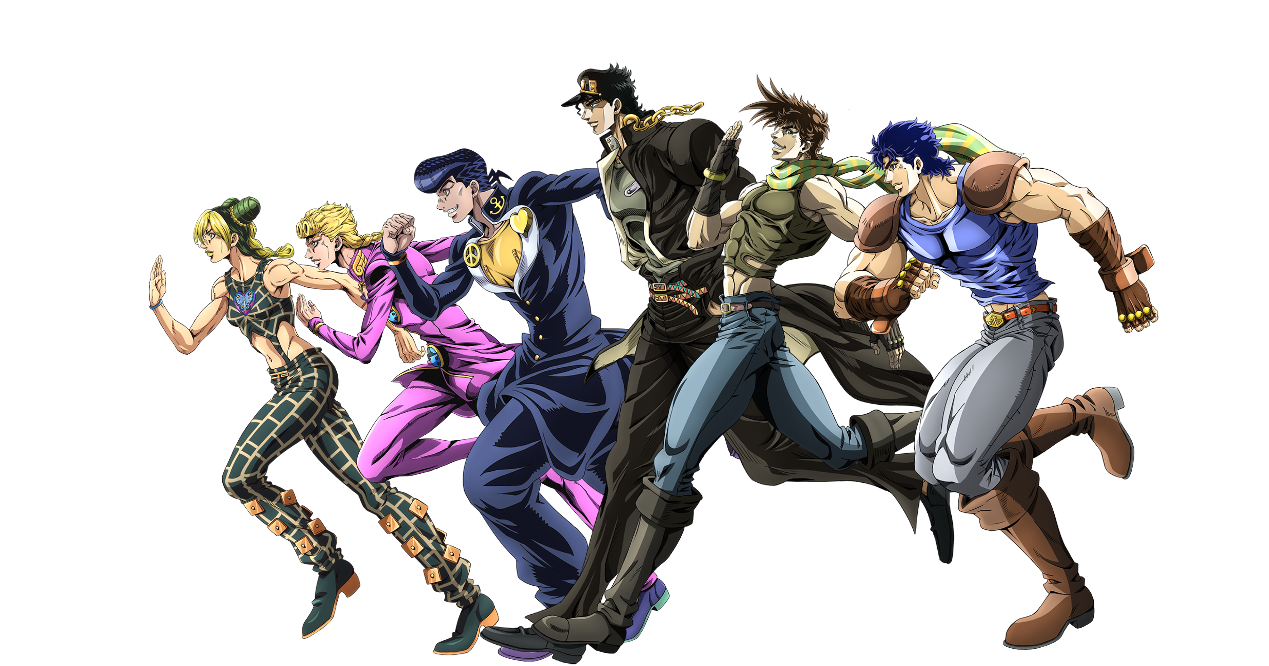
\includegraphics[width=\paperwidth,height=0.42\paperheight,keepaspectratio]{jojo-title-img.png}}

\title{JoJo's Bizarre Adventure}
\author{Nguyễn Duy Đạt}
\institute{HUST}
\date{\today}
% Remove something unused
\setbeamertemplate{footline}{%
\scriptsize{
}}

% Hide navigation bar
\setbeamertemplate{navigation symbols}{}

\begin{document}

% Title slide
\begin{frame}
	\titlepage
\end{frame}

% Table of contents
\AtBeginSection[]
{
	\begin{frame}
		\frametitle{Contents}
		\tableofcontents[currentsection]
	\end{frame}
}
\begin{frame}
	\frametitle{Table of Contents}
	\tableofcontents
\end{frame}
% Introduction slide
\section{Introduction}
\begin{frame}{Introduction}
	\begin{columns}[T]
		
		
		\begin{column}{0.45\textwidth}
			\begin{itemize}
				\item<1-> A Japanese manga and anime series.
				\vspace{1.5em}
				\item<1->
				Created by Hirohiko Araki, first debuted in 1987.
				\vspace{1.5em}
				\item<2-> Well-known for its unique art style and dynamic poses.
			\end{itemize}
		\end{column}
		
		\begin{column}{0.55\textwidth}
			\centering
			      
			\onslide<1->{
				\centering
				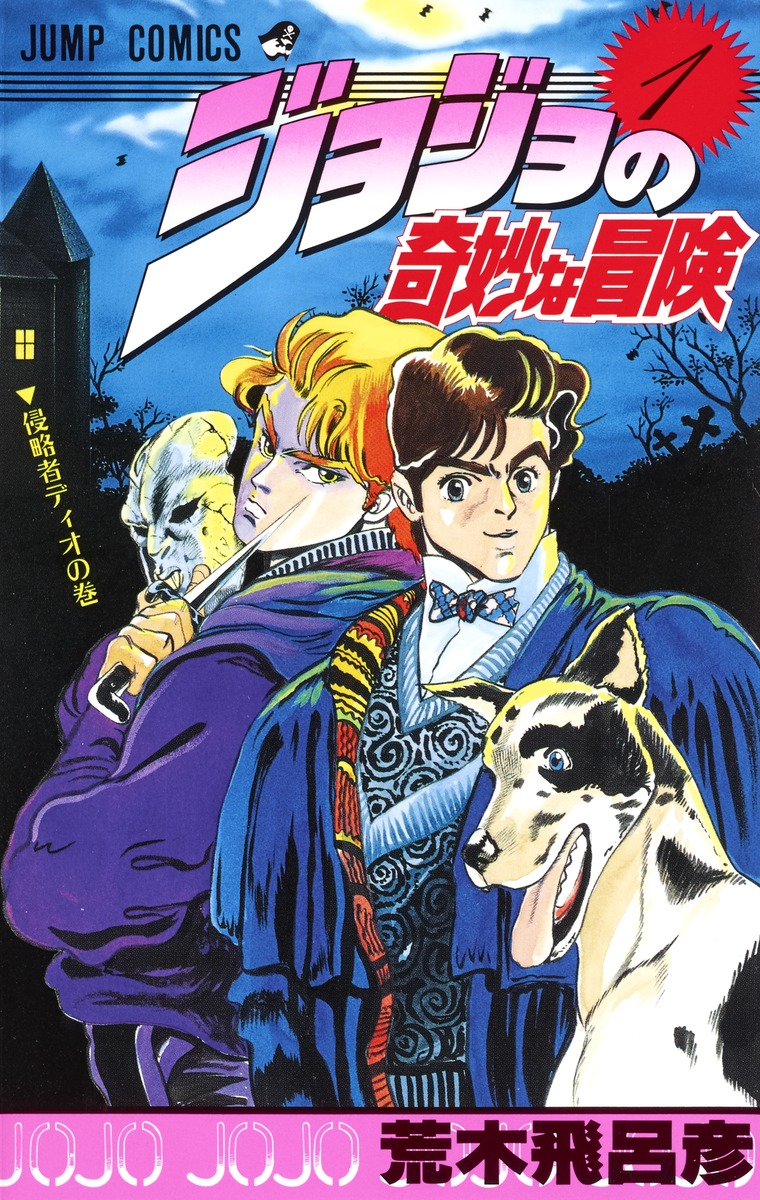
\includegraphics[height=0.34\textheight,width=\linewidth,keepaspectratio]{Volume_1.jpg}
				\hspace{0.6em}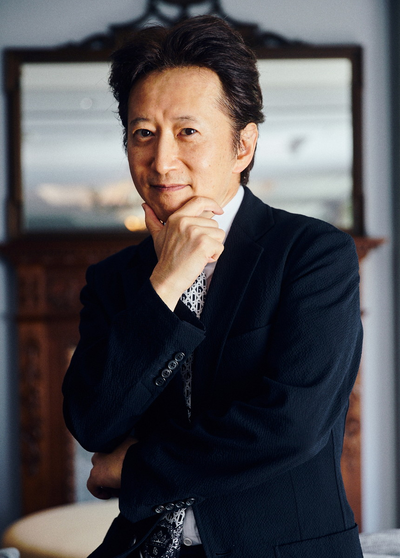
\includegraphics[height=0.34\textheight,width=\linewidth,keepaspectratio]{Hirohiko_Araki.png}
				\vspace{0.4em} 
			}
			
			\onslide<2->{
				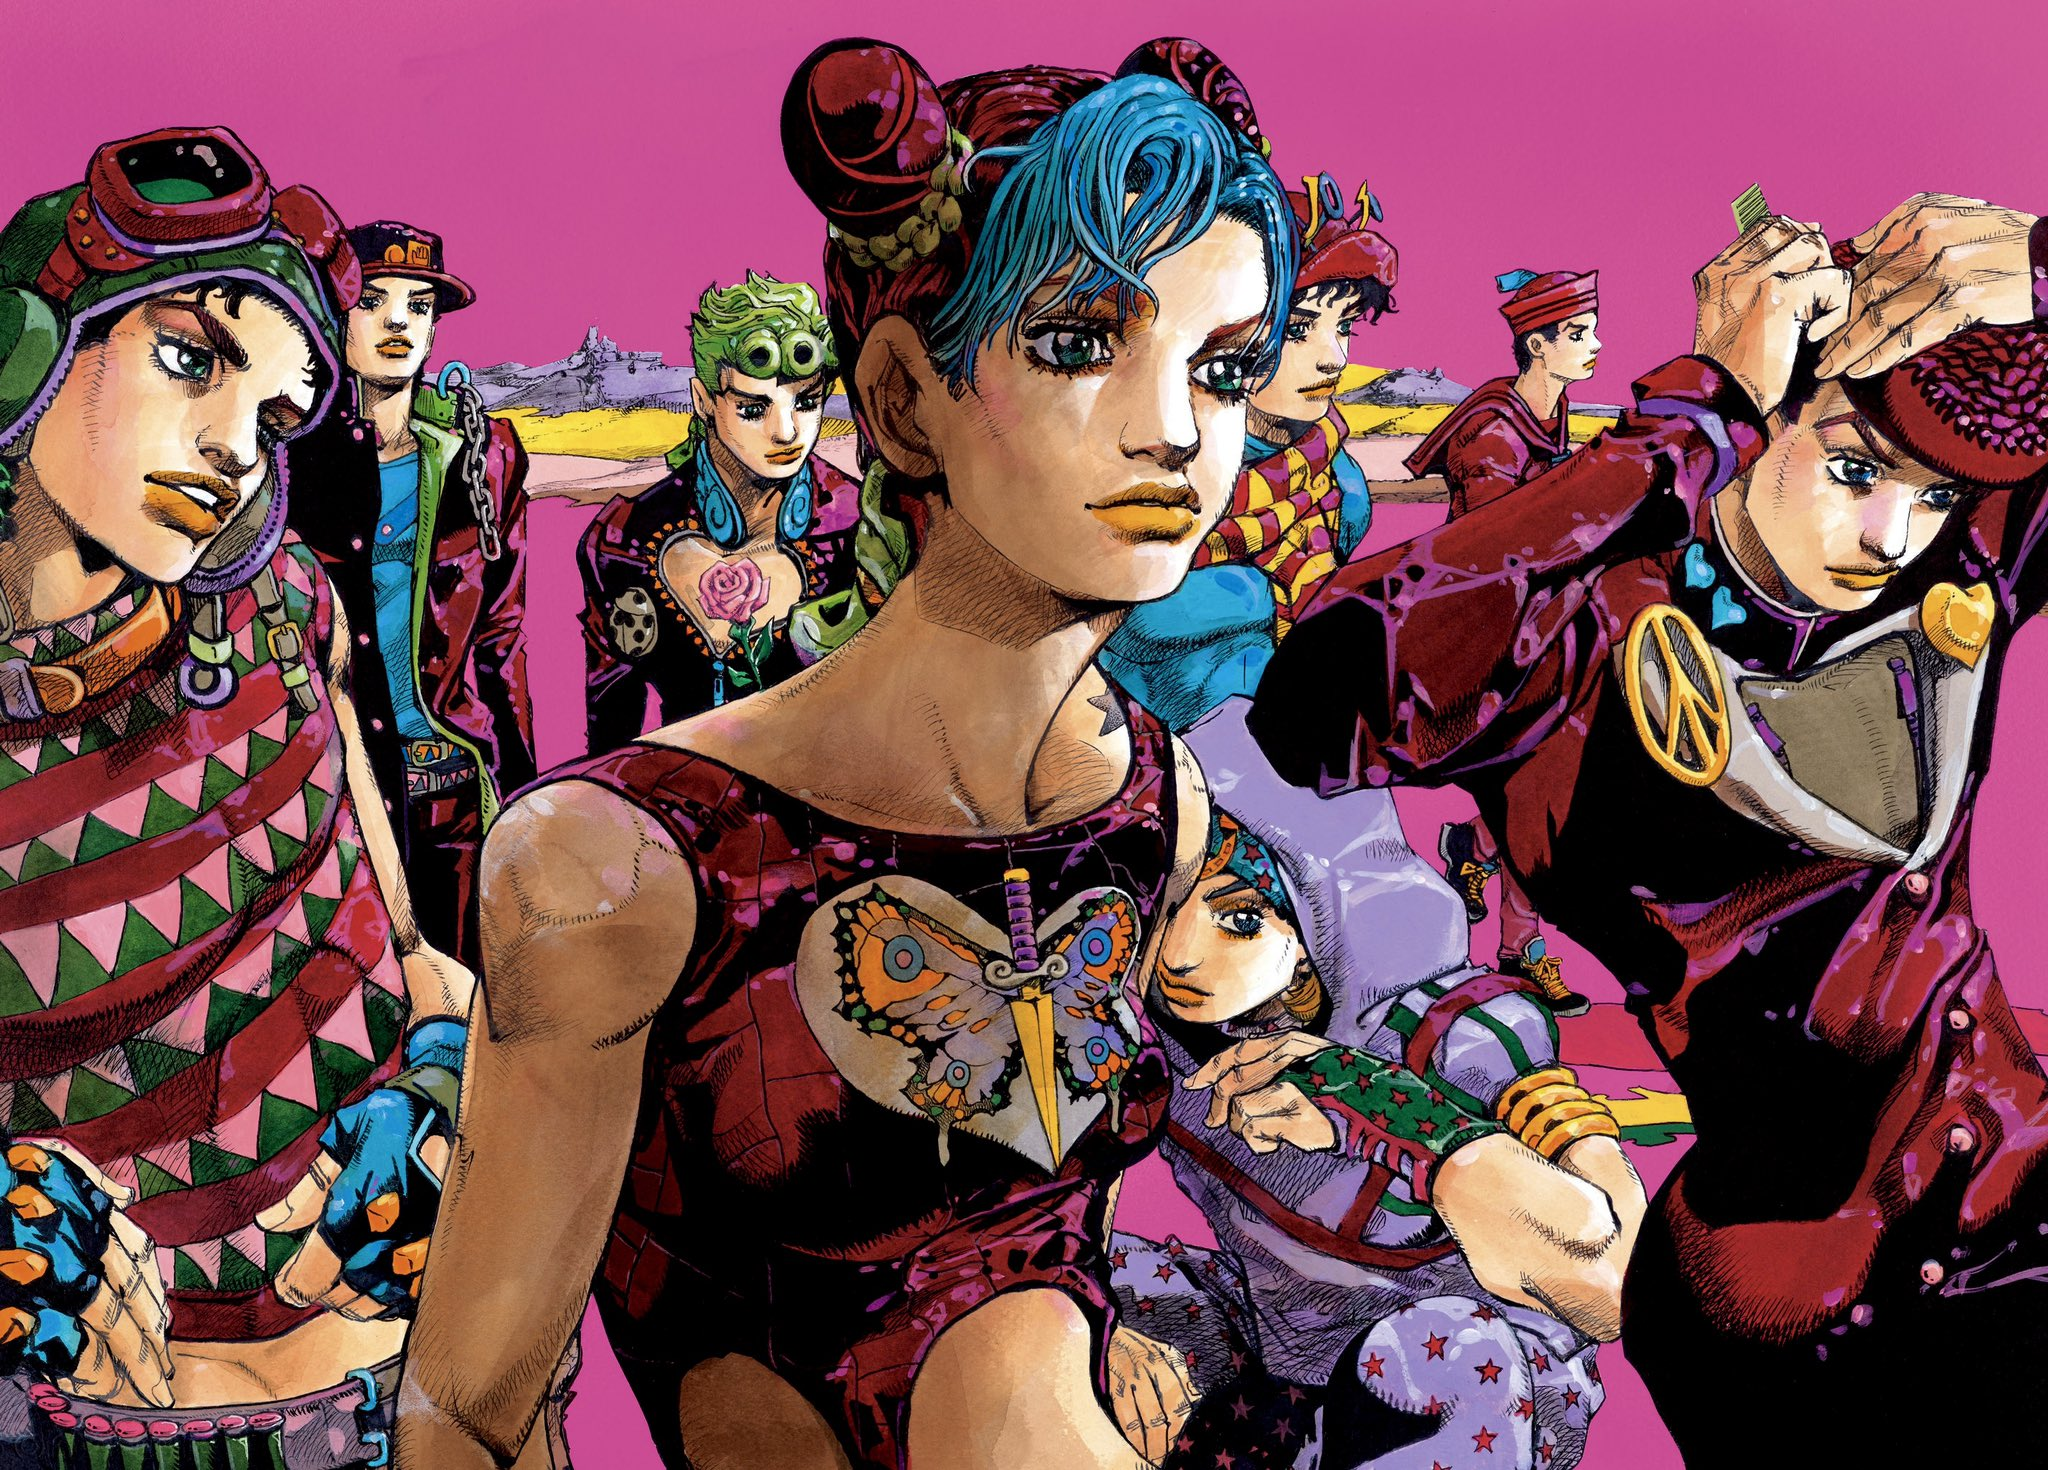
\includegraphics[height=0.5\textheight,width=\linewidth,keepaspectratio]{FpQ8mu7WcAEso0_.jpg}
			}
		\end{column}
		
	\end{columns}
\end{frame}

% Characters and abilities slide
\section{Characters and Powers}
\begin{frame}{Characters}
	\begin{columns}[T]
		
		
		\begin{column}{0.45\textwidth}
			\begin{itemize}
				\vspace{2em}
				\item<1-> Protagonists: Members of Joestar family
				\vspace{6.5em}
				\item<2-> Antagonists: Dio Brando, Pillar Men, Kira, \dots 
			\end{itemize}
		\end{column}
		
		\begin{column}{0.55\textwidth}
			\onslide<1->{
				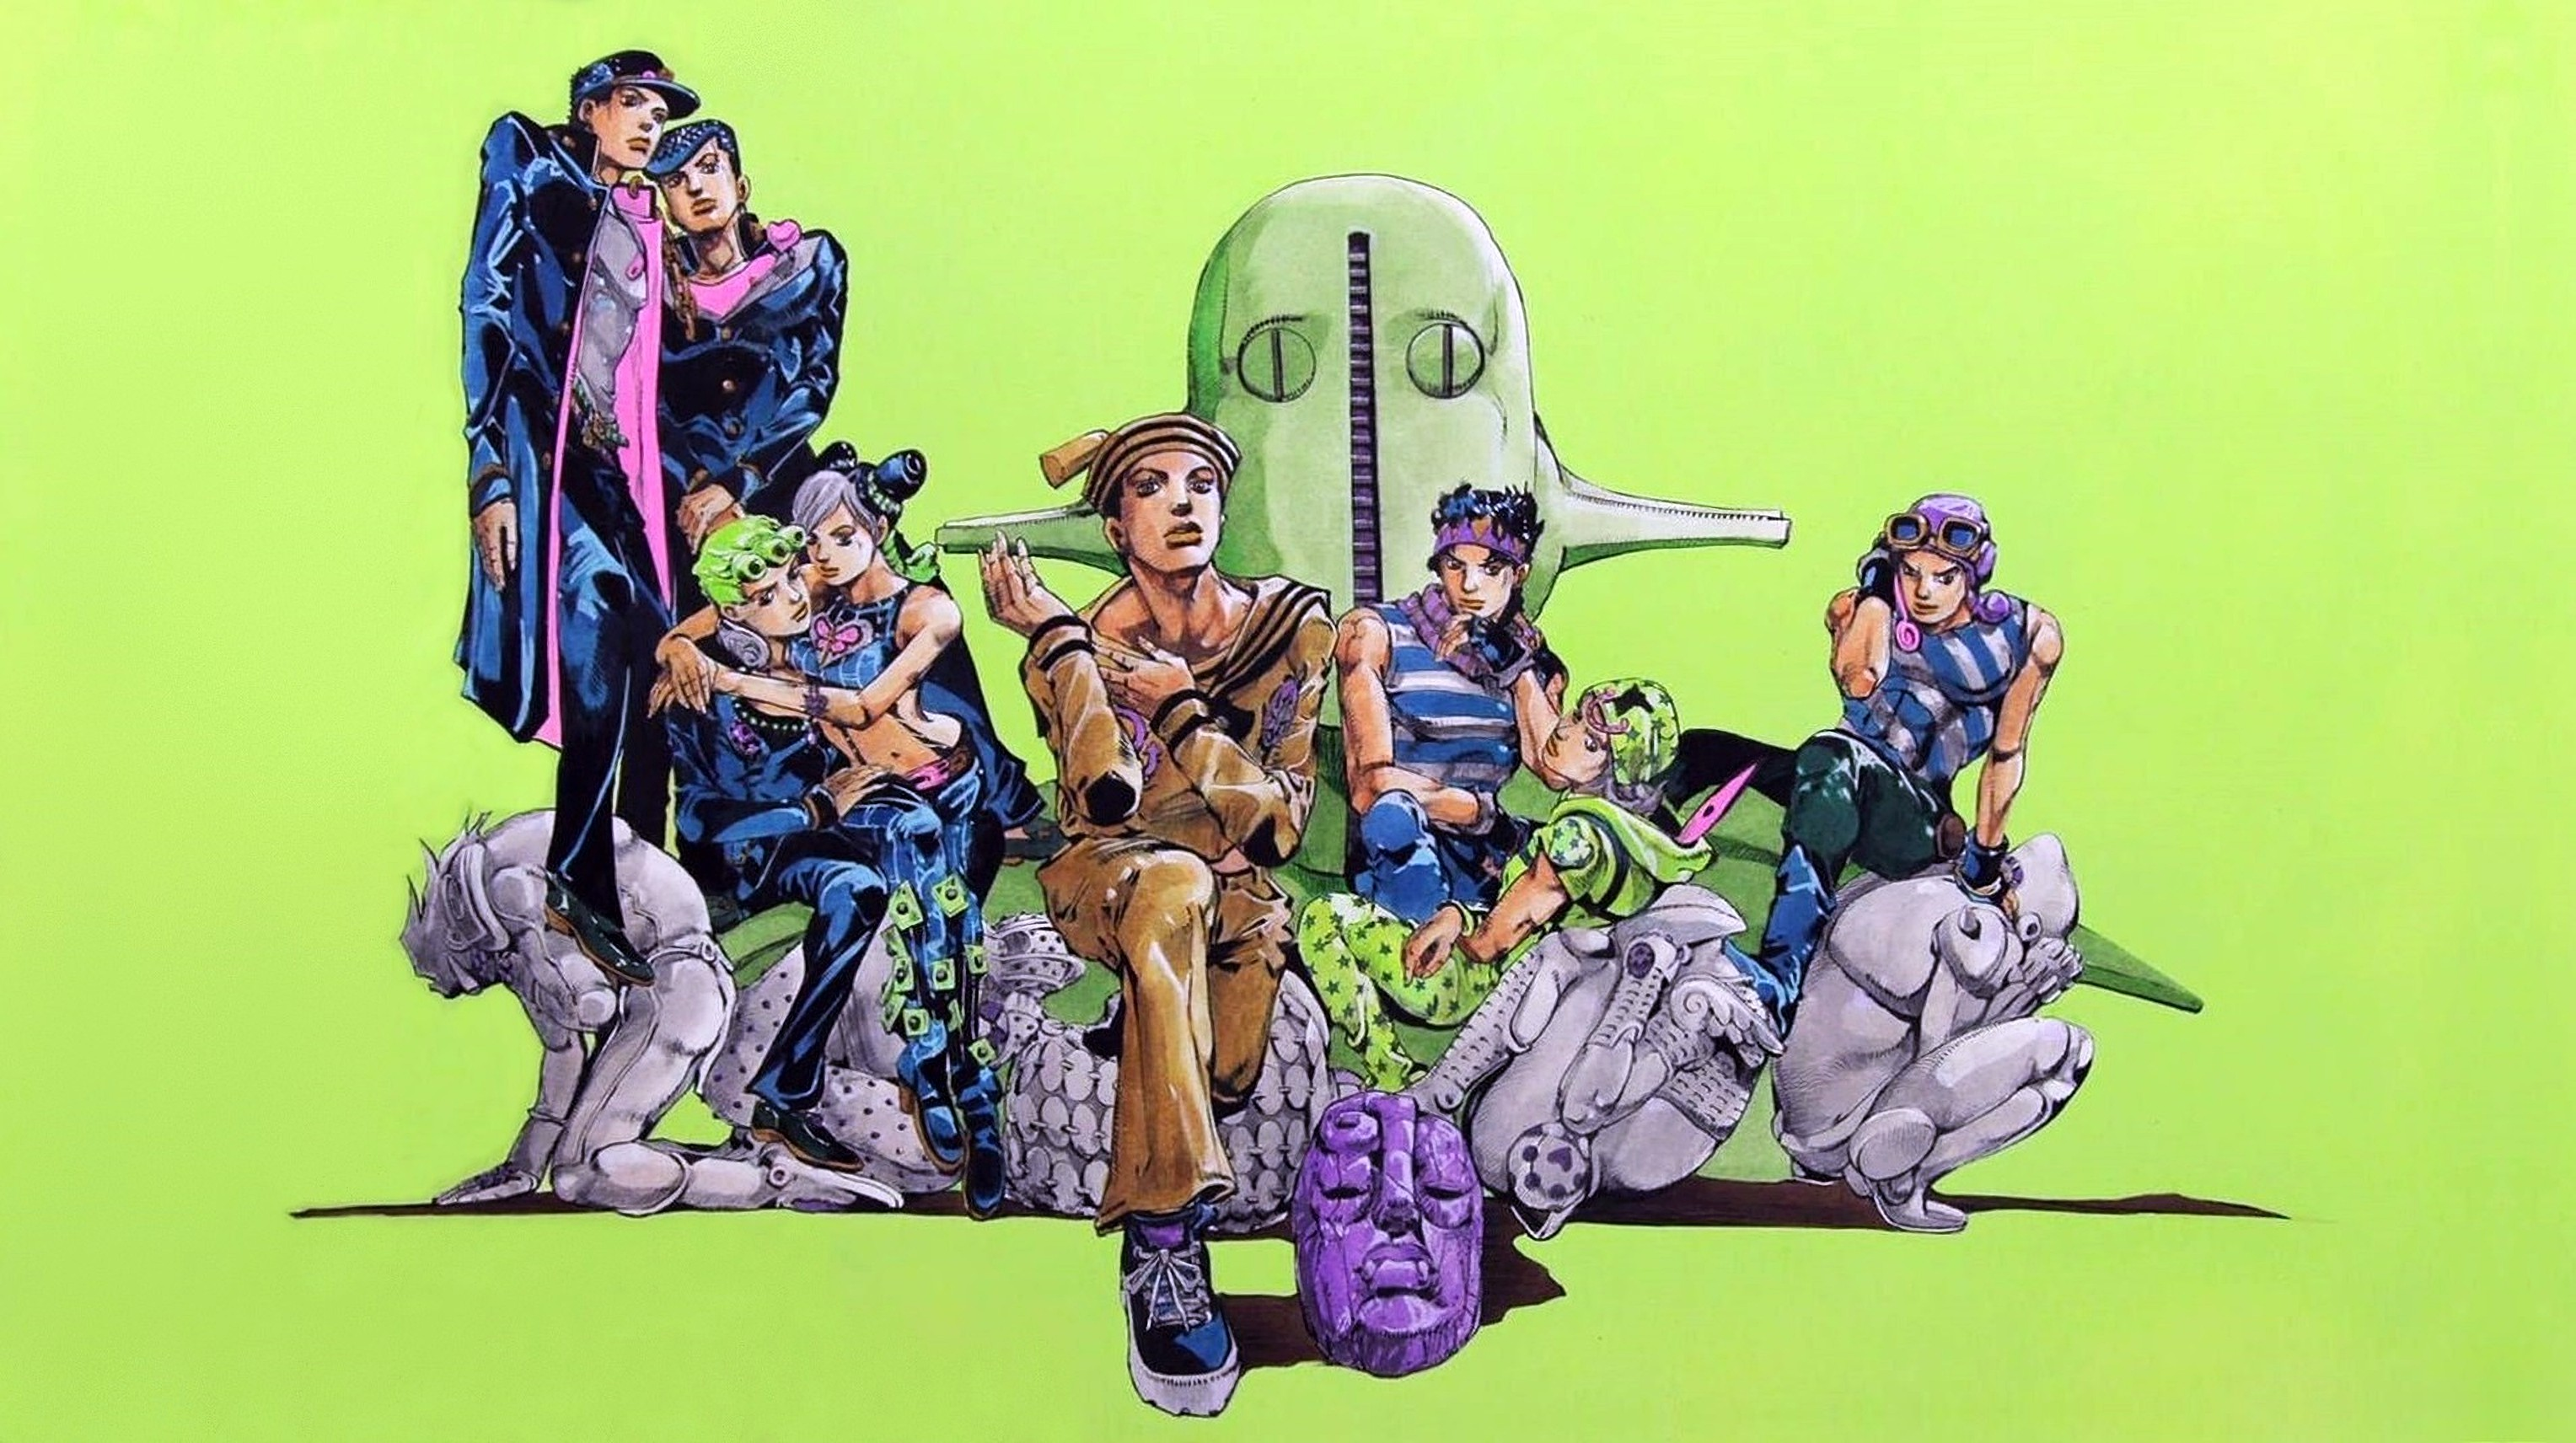
\includegraphics[height=0.5\textheight,width=\linewidth,keepaspectratio]{a0b.jpg}
			}
			
			\onslide<2->{
				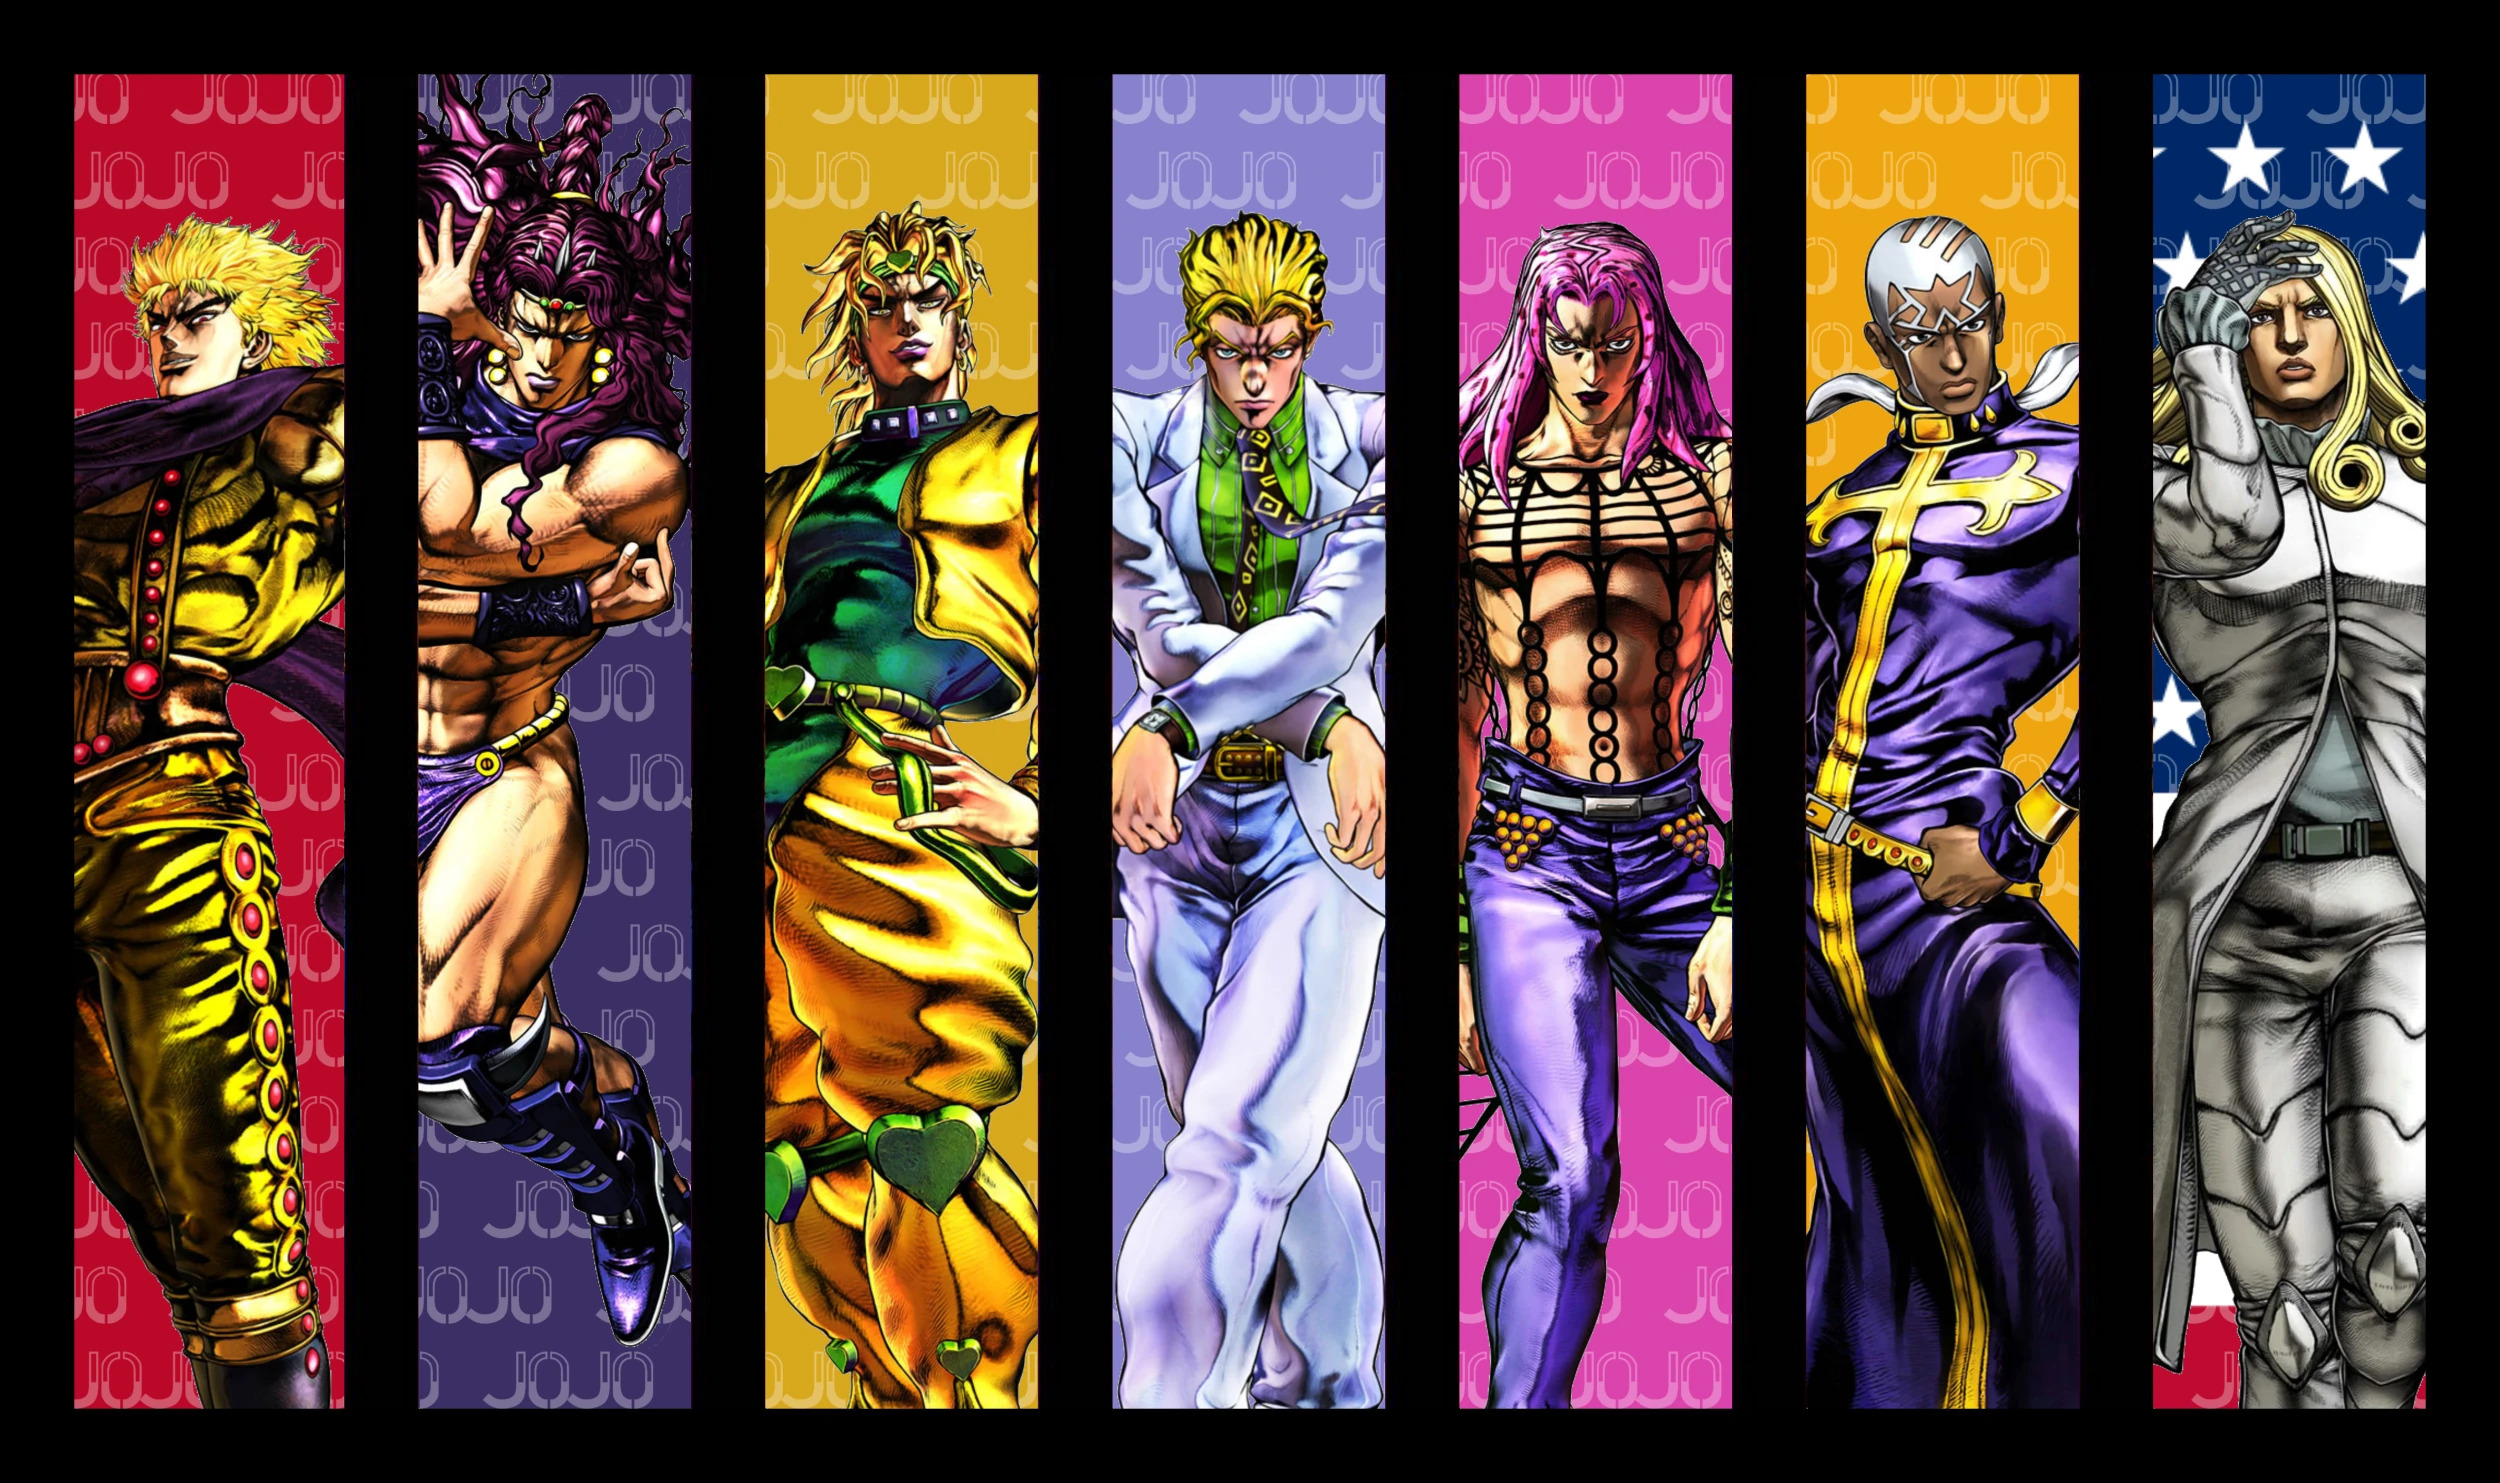
\includegraphics[height=0.5\textheight,width=\linewidth,keepaspectratio]{Jojo_villains.jpg}
			}
		\end{column}
		
	\end{columns}
\end{frame}
\begin{frame}{Powers}
	\begin{columns}[T]
		
		
		\begin{column}{0.45\textwidth}
			Hamon:
			\begin{itemize}
				\item<1-> Identical to Sun power.
				\item<1->Created by controlling breath.
				\vspace{6.5em}
			\end{itemize}
			\onslide<2->{
				Stand:
			}
			\begin{itemize}
				\item<2-> Power of spirit.
				\item<2-> Many shapes, sizes, have different abilities.
			\end{itemize}
		\end{column}
		
		\begin{column}{0.55\textwidth}
			\onslide<1->{
				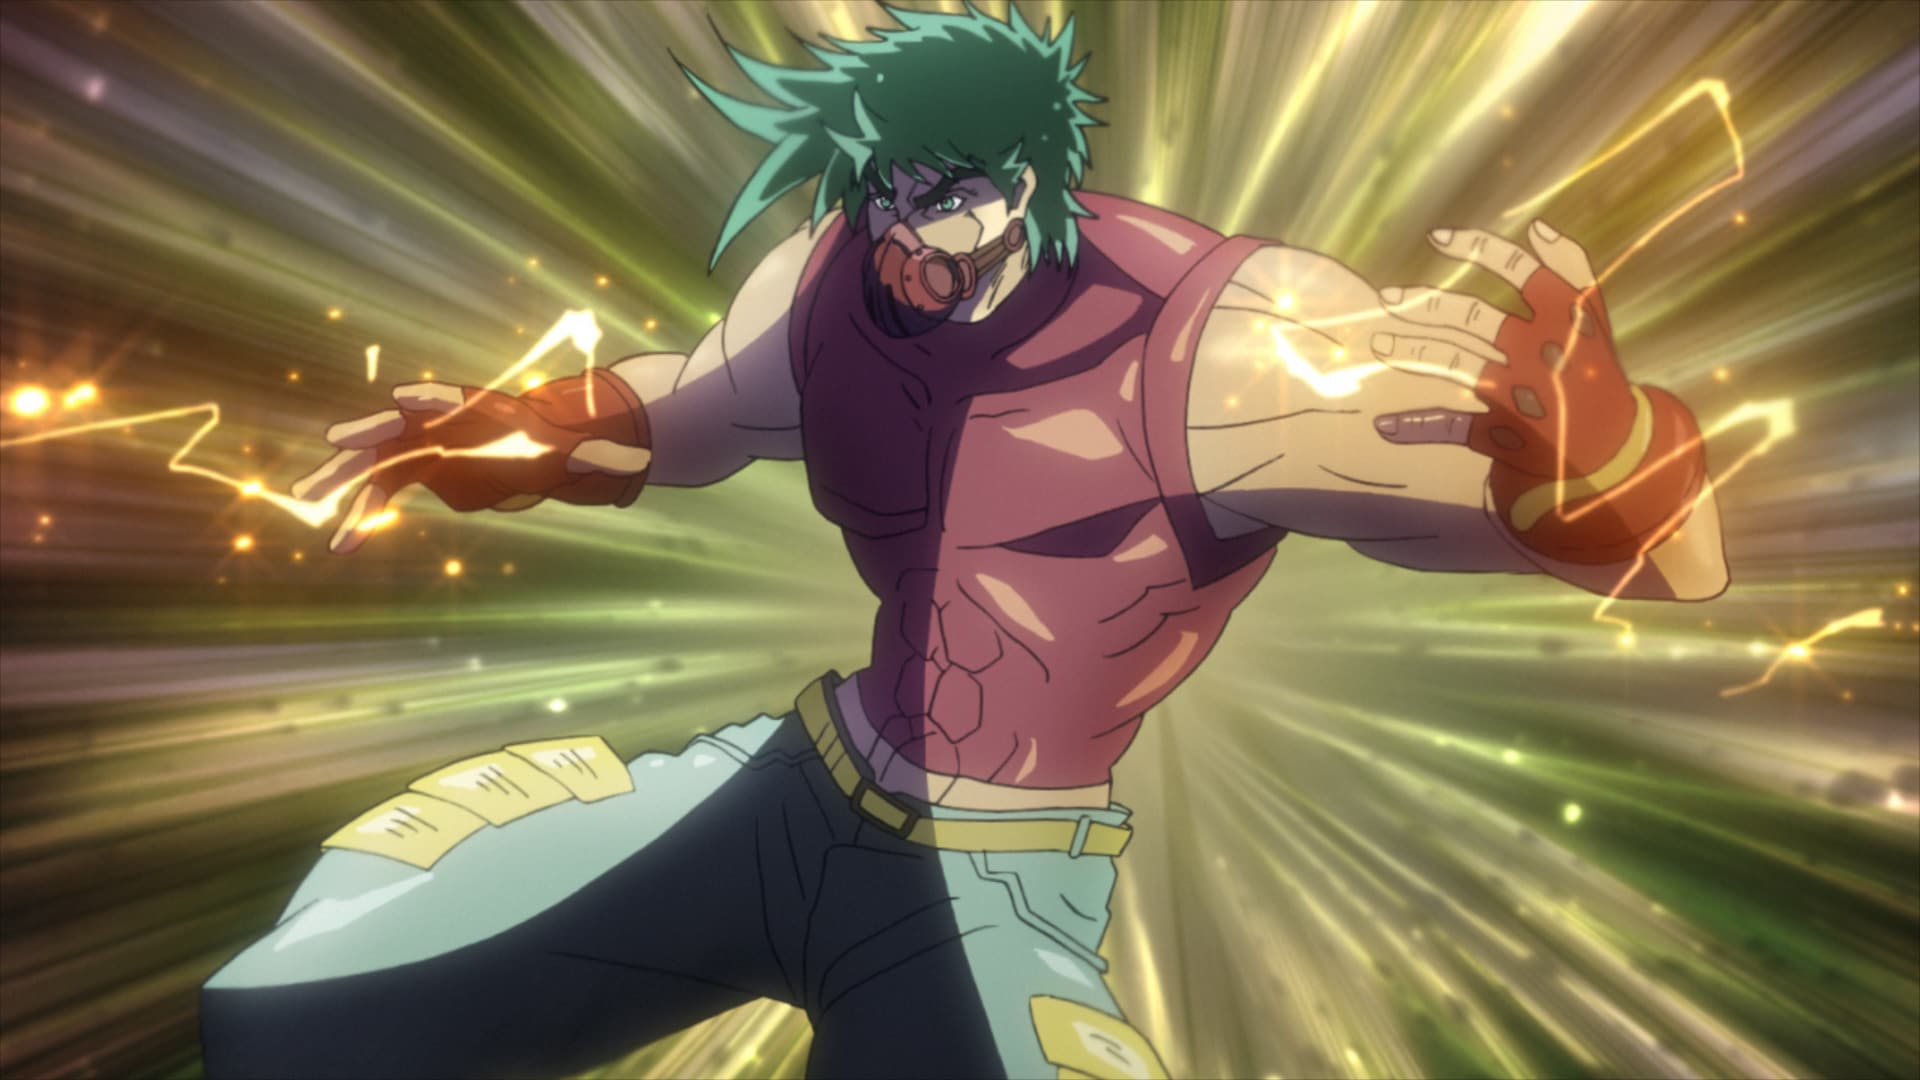
\includegraphics[height=0.5\textheight,width=\linewidth,keepaspectratio]{LAND_16_9.jpg}
			}
			\centering
			      
			\onslide<2->{
				\centering
				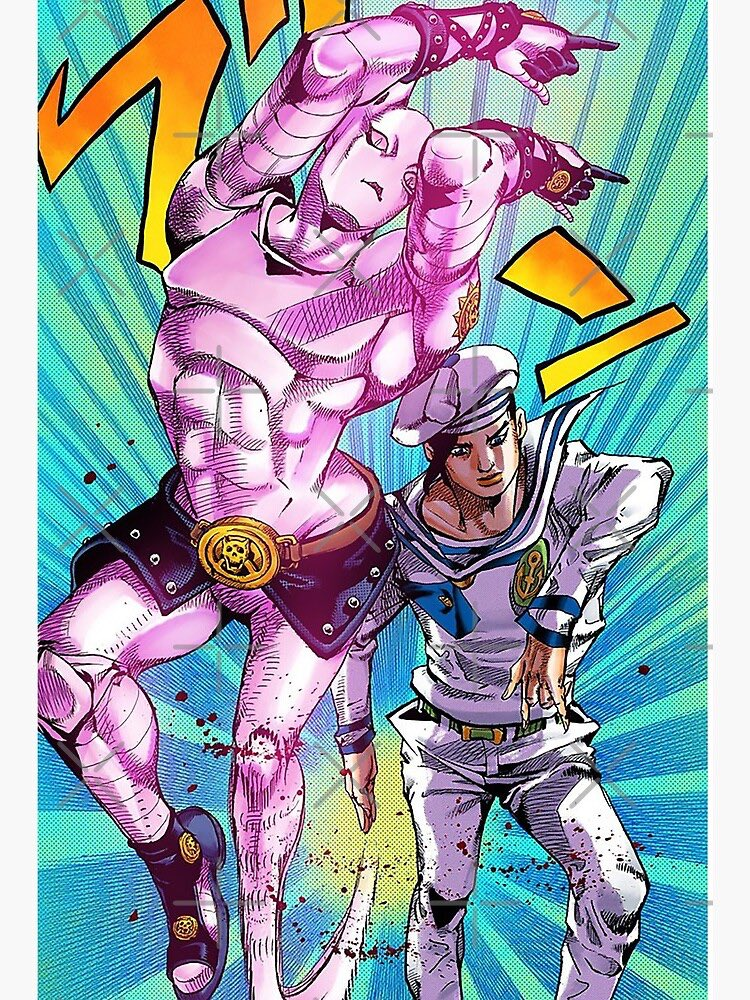
\includegraphics[height=0.36\textheight,width=\linewidth,keepaspectratio]{bd8a1a274ff7ec5fdcb94f1e0c0d6266.png}
				\hspace{0.6em}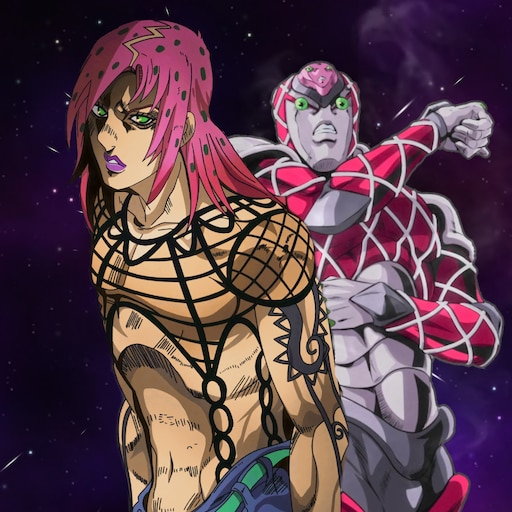
\includegraphics[height=0.36\textheight,width=\linewidth,keepaspectratio]{9l6amonnfzy91.jpg}
			}
			
			
		\end{column}
		
	\end{columns}
\end{frame}
% Cultural impact slide
\section{Cultural Impact}

%   \begin{itemize}
%     \item Inspiring bands and fashion designers.
%     \item Massive following of fans.
%     \item Numerous fan translations and fan-made content.
%   \end{itemize}
\begin{frame}{Cultural Impact}
	\begin{columns}[T]
		
		
		\begin{column}{0.45\textwidth}
			\begin{itemize}
				\item<1-> Fashion: inspire many collections.
				\vspace{1.5em}
				\item<1->
				Music: Numerous references throughout the series.
				\vspace{1.7em}
				\item<2->Fanbase: Passionate, many fan-made contents and events.
			\end{itemize}
		\end{column}
		
		\begin{column}{0.55\textwidth}
			\centering
			      
			\onslide<1->{
				\centering
				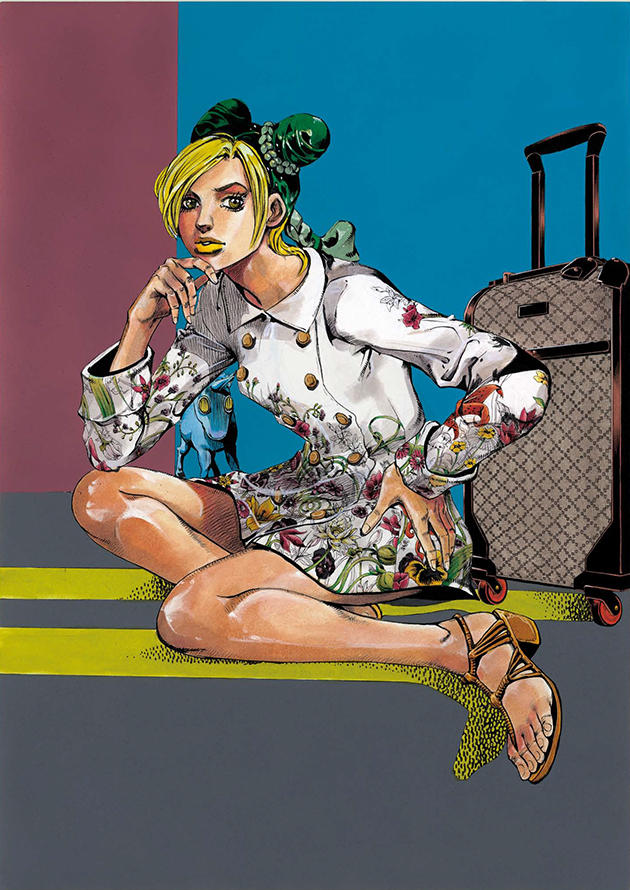
\includegraphics[height=0.38\textheight,width=\linewidth,keepaspectratio]{Jojo_Gucci4_splsh.jpg}
				\hspace{0.6em}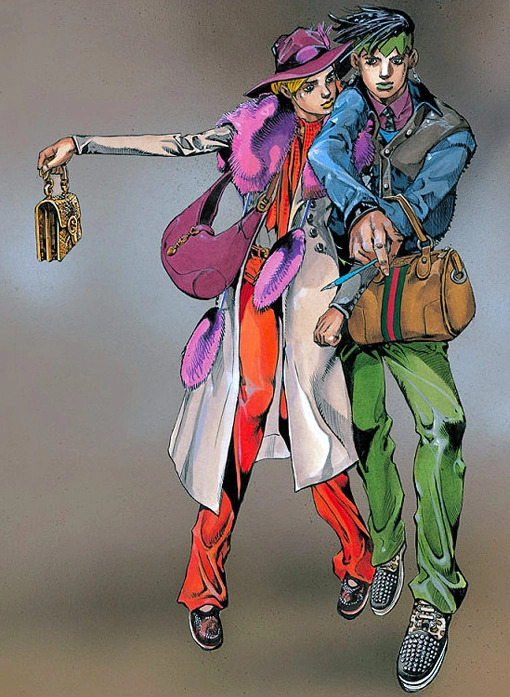
\includegraphics[height=0.38\textheight,width=\linewidth,keepaspectratio]{Gucci_X_Araki_X_Spur.jpg}
				\vspace{0.4em} 
			}
			
			\onslide<2->{
				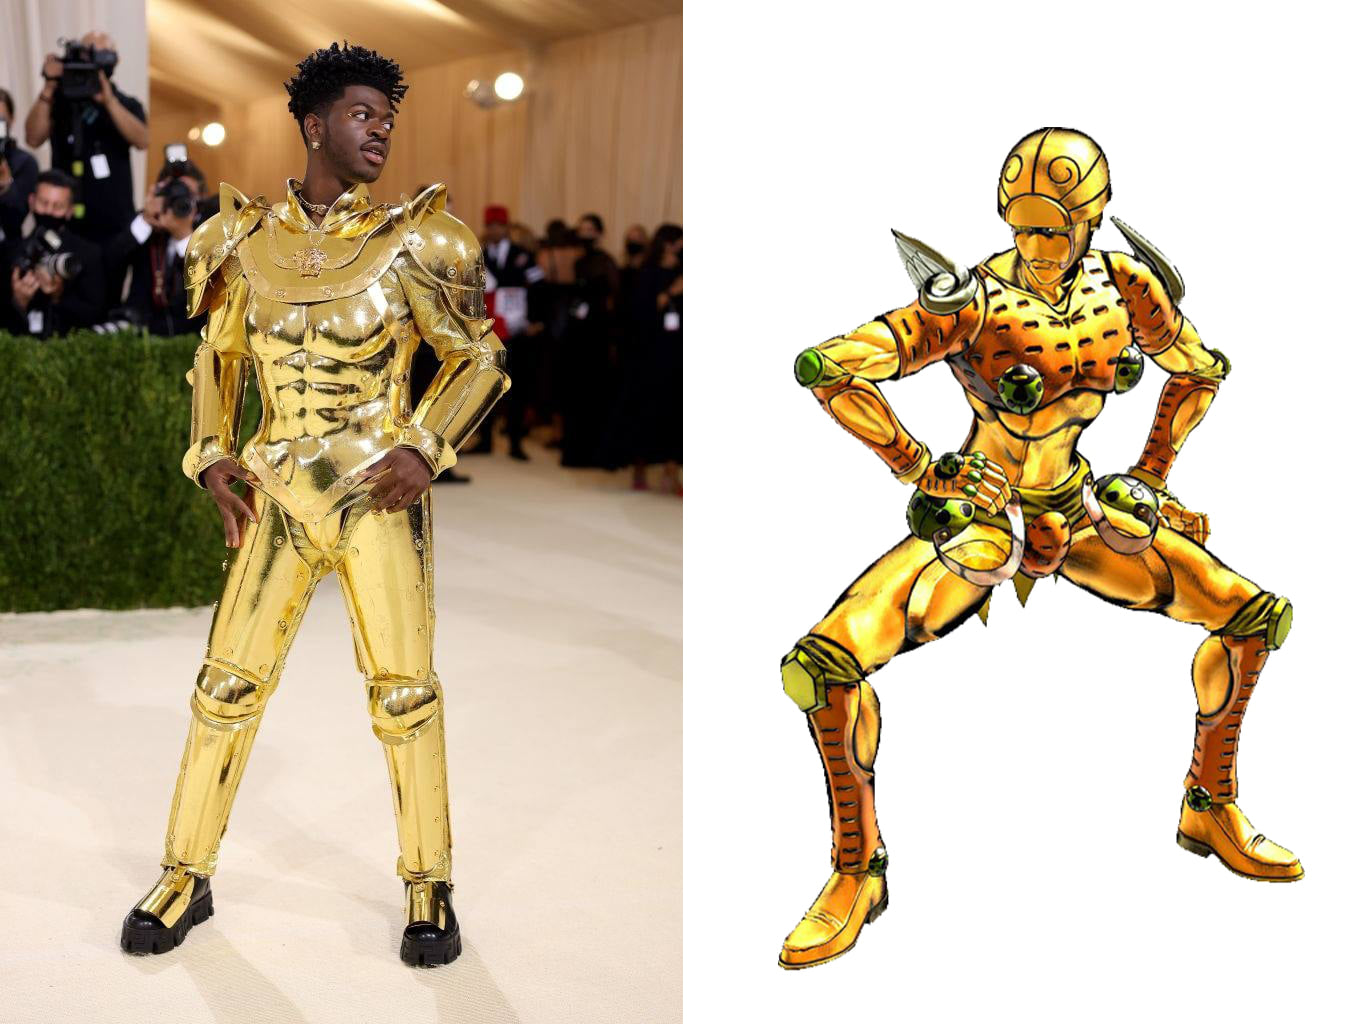
\includegraphics[height=0.43\textheight,width=1.2\linewidth,keepaspectratio]{240601833_4251106004924736_755389383533408688_n.jpg}
			}
		\end{column}
		
	\end{columns}
\end{frame}
% Conclusion slide
\section{Conclusion}
\begin{frame}{Conclusion}
	\begin{itemize}
		\item Highly influential and iconic series.
		      \vspace{1em}
		\item Diverse cast of characters.
		      \vspace{1em}
		\item Cultural phenomenon.
	\end{itemize}
\end{frame}
\begin{frame}{References}
	\begin{thebibliography}{9}
		\bibitem{wiki} 
		Wikipedia: JoJo's Bizarre Adventure.
		\\\url{https://en.wikipedia.org/wiki/JoJo\%27s\_Bizarre\_Adventure}
		    
		\bibitem{wiki} 
		JoJo's Bizarre Wiki.
		\\\url{https://jojo.fandom.com/wiki/Main\_Page}
		    
		\bibitem{jojoanime10th}
		\emph{Jojo Anime 10th Anniversary Project.}\\
		\url{https://jojoanime10th.com/}.
		    
		\bibitem{anime} 
		David Production. 
		\textit{JoJo's Bizarre Adventure (TV Series)}.\\
		\bibitem{more}
		and more.
	\end{thebibliography}
\end{frame}

\end{document}